
En esta sección se trabajó con el conjunto de datos registrados por el arreglo principal con Todos los Disparos. Las características de estos datos se resumen en la Tabla~\ref{tabla:caracteristicas_ALL} La señal de $S(1000)$ de este conjunto fue corregida en la reconstrucción oficial de eventos por la modulación del clima, por los parámetros obtenidos en \cite{aab2017impact}.

\begin{table}[H]
  \centering
  \begin{tabular}{|c|c|}
  \hline
  Inicio              & 01  de Enero de 2014\\ \hline
  Final               & 01  de Enero de 2020       							\\ \hline
  Número de eventos   & 1\,263\,015							\\ \hline 
  Energía media       & 1.76\,EeV       				\\ \hline  %  1.005\,EeV
  Corte en $S_{38}$   & 5.36 VEM        				\\ \hline 
  Corte en ángulo cenital		  & $\theta < 60^o$ 				\\ \hline
  \end{tabular}
\caption{Características del conjunto de datos de Todos los Disparos.} \label{tabla:caracteristicas_ALL}
\end{table}


% \begin{figure}[H]
%   \centering
%   \begin{subfigure}[b]{0.9\textwidth}
%   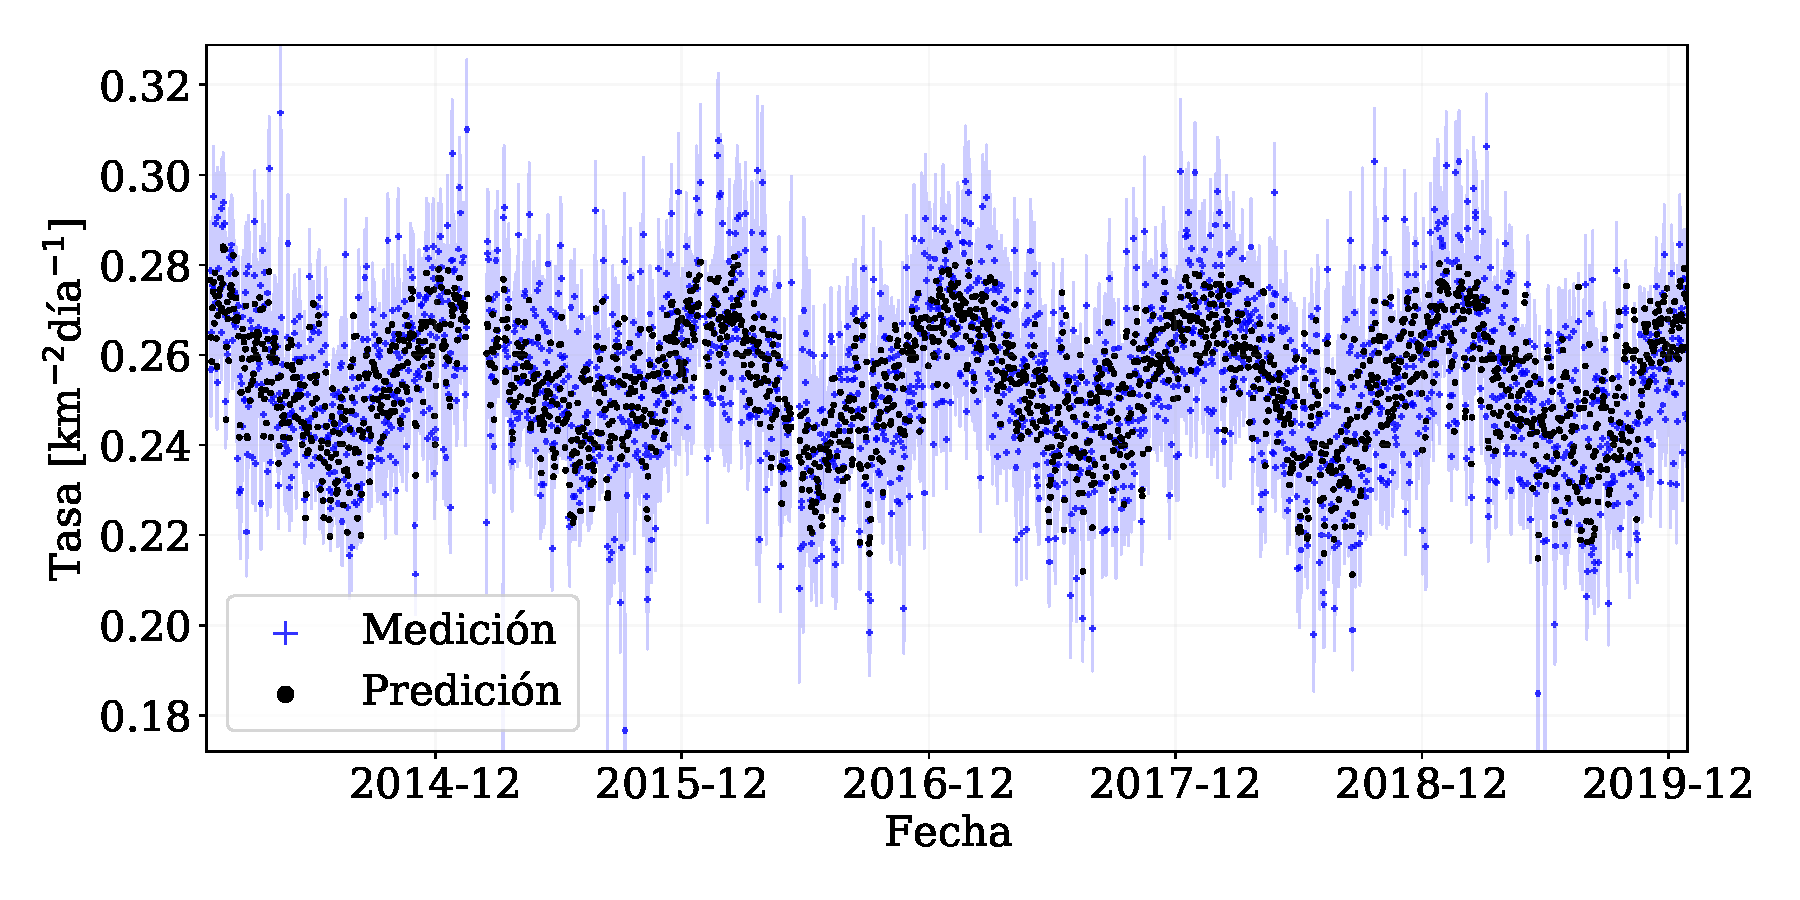
\includegraphics[width=\textwidth]{../04_Clima/Graphs/rate_dayly/AllTriggers_S38_over_1EeV_rate_v3.pdf}
%   \caption{Tasa eventos por día}\label{fig:rate_dayly_AllTriggers}
%   \end{subfigure}\\
%   % \hspace{\fill}
%   \begin{subfigure}[b]{0.9\textwidth}
%   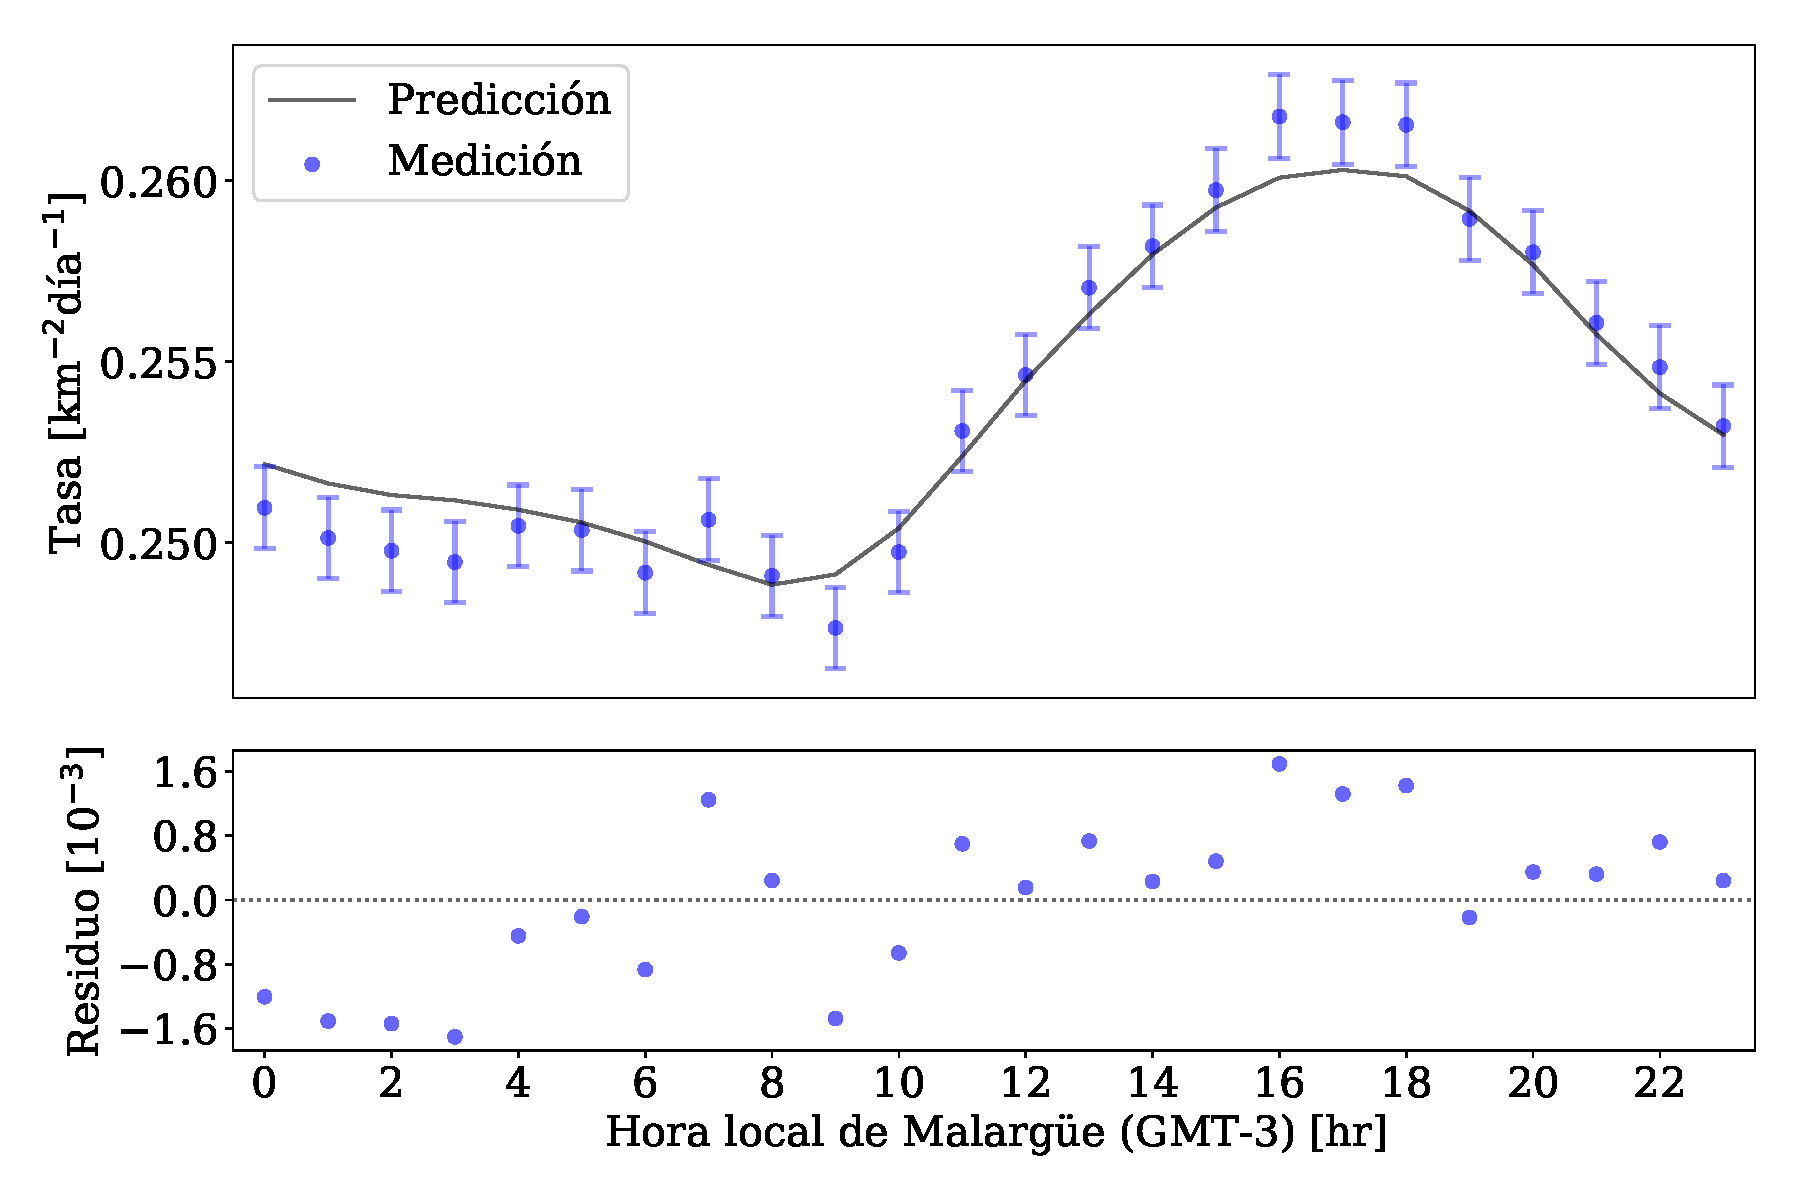
\includegraphics[width=\textwidth]{../04_Clima/Graphs/rate_hour_of_the_day/AllTriggers_S38_over_1EeV_hour_of_the_day.pdf}
%   \caption{Tasa de eventos promediada por hora del día }\label{fig:rate_hod_AllTriggers}
%   \end{subfigure}%
%   \caption{Tasa de eventos por días comparadas con el ajuste entre los años 2005 hasta 2015. Los datos analizados fueron los presentados en la ICRC 2015 para energías mayores a $1\,$EeV donde se observa la modulación anual y diaria del clima. }\label{fig:rate__AllTriggers}


En este trabajo se busca comparar los parámetros obtenidos con los eventos de Todos los Disparos con los parámetros de la reconstrucción oficial. Para esto se realizó un análisis con los datos de nueva reconstrucción de la señal $S_{38}$ sin la corrección del clima, siguiendo un proceso similar a la sección \ref{sin_corregir_s38}.

\subsection{Pesos de los hexágonos en el rango 2014-2020}

Para constatar que no exista ninguna anomalía en los pesos de los hexágonos, se realiza el cálculo de los mismos para tres frecuencias de referencia para el análisis de anisotropías.  Los pesos se muestran en la Fig.\,\ref{fig:wei_14_20}. El rango de tiempo en el que se calculan estas curvas es entre 1 de Enero del 2014 y el 1 de Enero del 2020.

\begin{figure}[H]
	\centering
	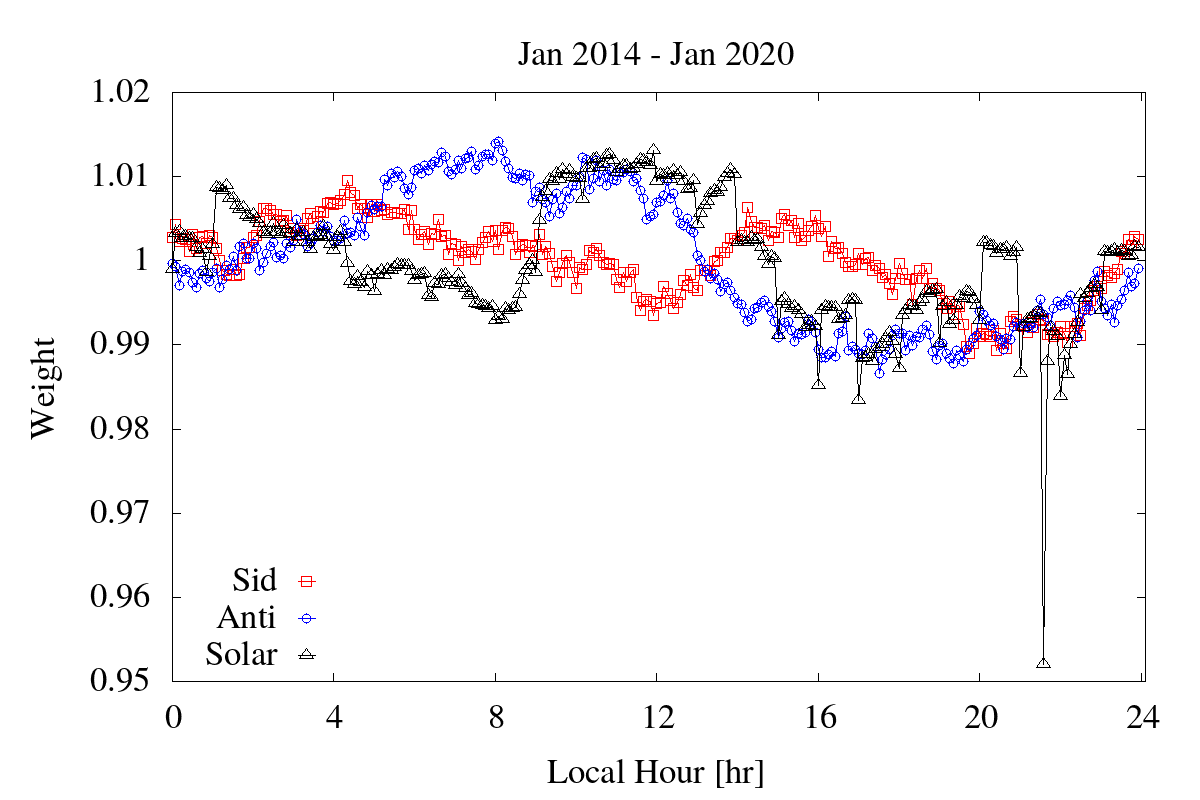
\includegraphics[width=0.5\textwidth]{weigth2014-2020_jan.png} 	
	\caption{Pesos de los hexágonos}
	\label{fig:wei_14_20}
\end{figure}



      Considerando el filtro con el S38 en el archivo 2020 y la energía en el 2017, quiero saber si obtengo parámetros  del clima comparables. Ya que el Main Array se corresponden los parámetros del 2015 y 2019, yo esperaría que con todos los triggers pase los mismo. Una diferencia importante entre ambos análisis es que los parámetros del 2020 contienen eventos hasta el 31/12/2019.
      
      Los mismos se comparan con los ajustes obtenidos en \cite{aab2017impact}.

        \begin{figure}[H]
          \centering
          \begin{subfigure}[b]{0.8\textwidth}
          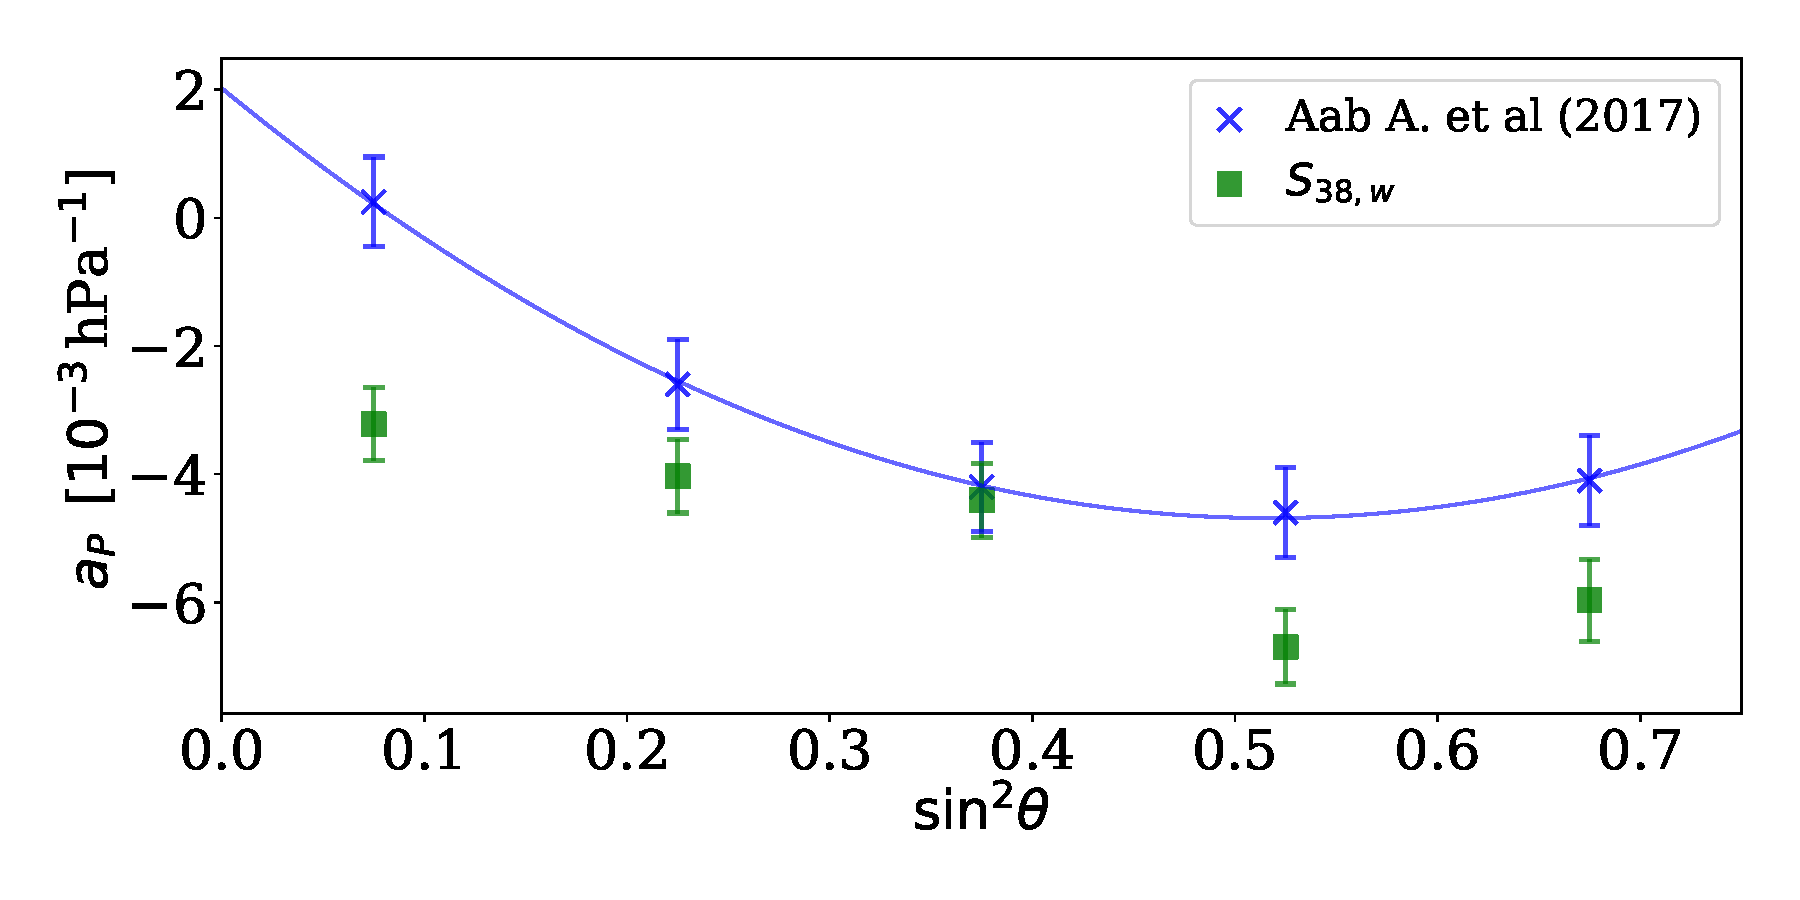
\includegraphics[width=\linewidth]{../04_Clima/Graphs/params/ap_AllTriggers.pdf}
          \caption{Parámetro $a_P$ }
          \end{subfigure}\\
          \begin{subfigure}[b]{0.8\textwidth}
          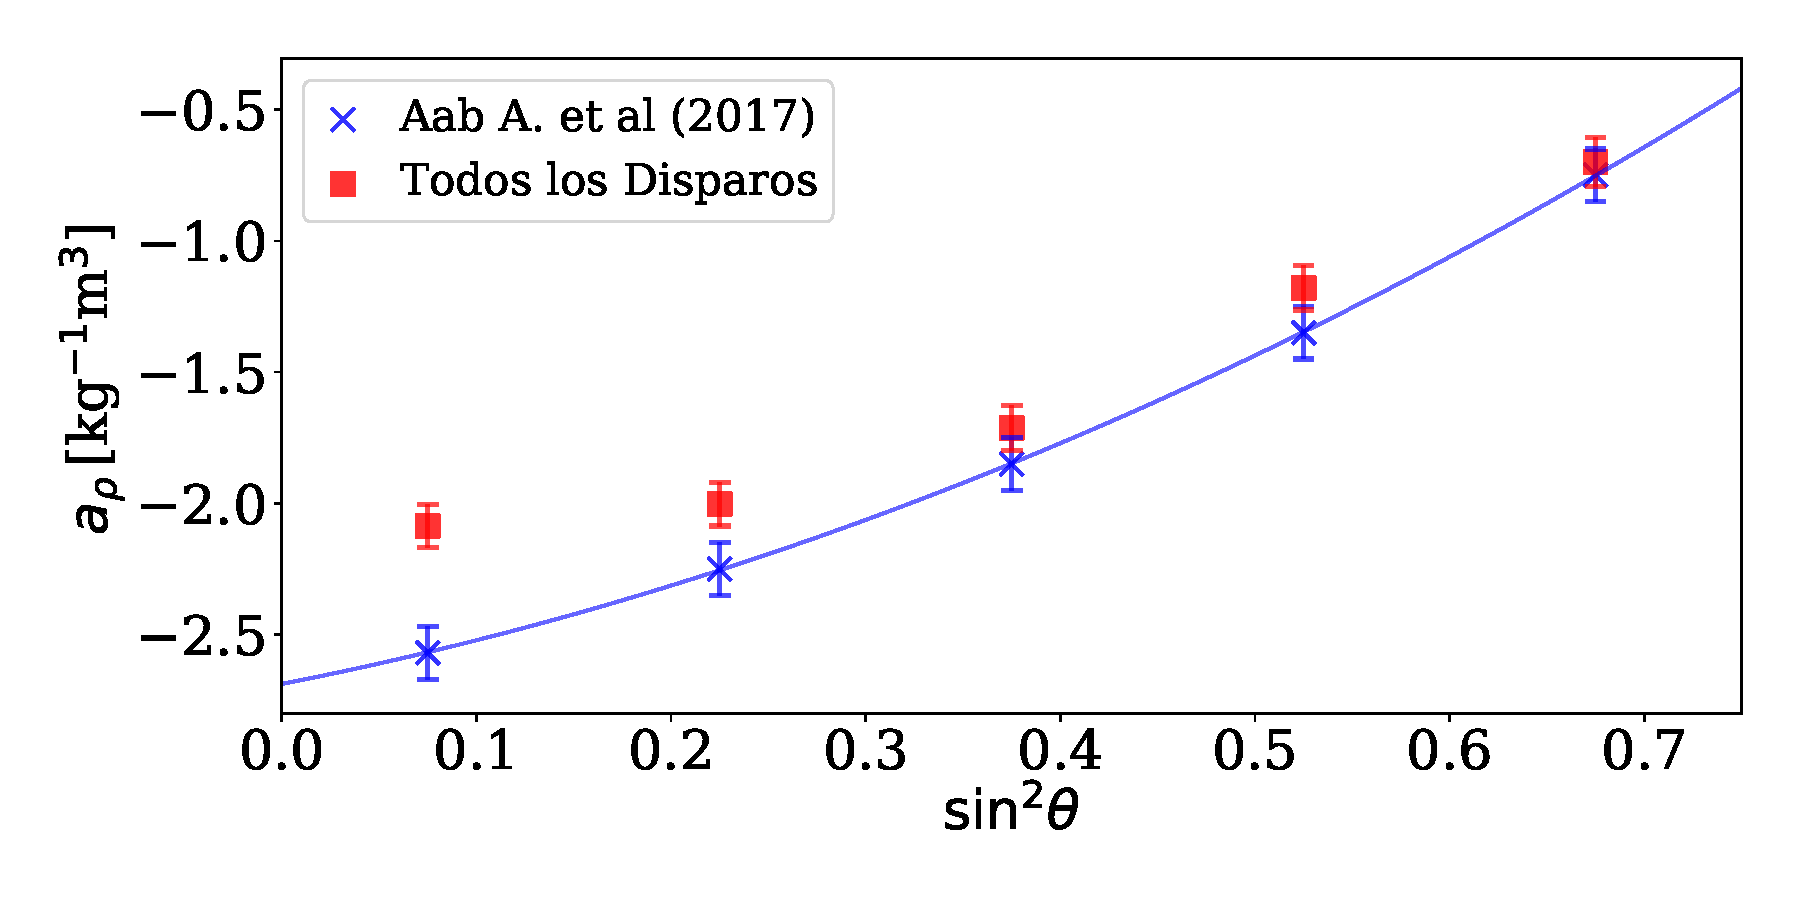
\includegraphics[width=\linewidth]{../04_Clima/Graphs/params/arho_AllTriggers.pdf}
          \caption{Parámetro $a_{\rho}$ }
          \end{subfigure}\\
          \begin{subfigure}[b]{\textwidth}
          \centering
          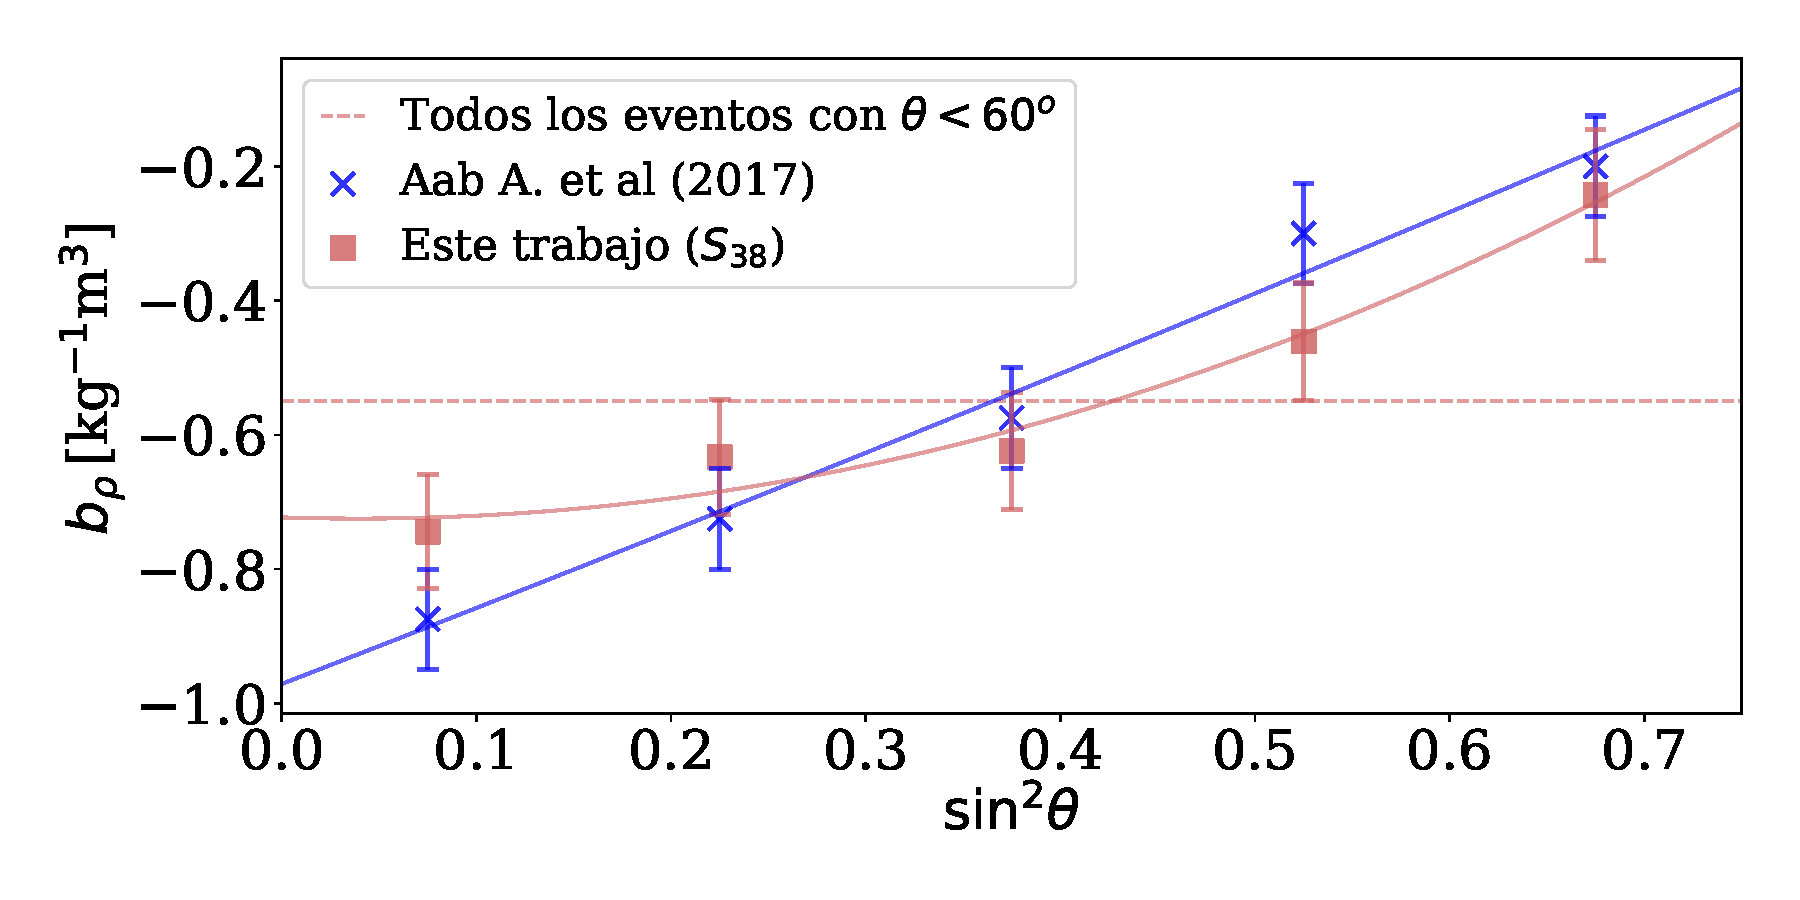
\includegraphics[width=0.8\linewidth]{../04_Clima/Graphs/params/brho_AllTriggers.pdf}
          \caption{Parámetro  $b_\rho$   }
          \end{subfigure}
          \caption{Parámetros de la modulación del clima considerando los datos para todos los disparos del archivo 2017 y 2020. Los mismos se comparan con los coeficientes utilizados por la Colaboración.}
        \end{figure}

%       ???????????Se ve que estos parámetros no son comparables. 
